\section{由有限表示构造覆盖}
\label{sec:fcover-finite-representations}

第~\ref{chap:functions-as-vectors}章说过，一个函数有两种“一列数”：取值列，下标是输入；系数列，下标是基函数的编号。上一节截取的是取值列，节点数随精度增长。本节换成系数列：若整类函数都能用同一组有限个基函数统一逼近，只是各自的系数不同，靠后的系数就可以整体舍去，覆盖问题分成两步，先把每个成员换成有限维子空间中的近似，再覆盖这些近似组成的有限维有界集。

\paragraph{统一逼近与有限维球}

设$(E,\lVert\cdot\rVert)$是实赋范函数空间，$V\subseteq E$是$n$维子空间。第~\ref{chap:metric-spaces}章证明了：在$n$维实赋范空间中，半径$R$的闭球可以被至多$(1+2R/\varepsilon_1)^n$个半径$\varepsilon_1$的闭球覆盖，中心取在该空间内。这就是立方体计数式~\eqref{eq:fcover-cube}的一般形式。把它用于$V$及$E$限制在$V$上的范数，就得到下面的结论。

\begin{theorem}[有限维统一逼近给出覆盖]
\label{thm:fcover-finite-dimensional}
设$\mathcal F\subseteq E$，$\varepsilon_0\geq0$，$R>0$。若对每个$f\in\mathcal F$都存在$g_f\in V$，使
\begin{equation}
 \lVert f-g_f\rVert\leq\varepsilon_0,\qquad\lVert g_f\rVert\leq R,
 \label{eq:fcover-uniform-approximation}
\end{equation}
则对每个$\varepsilon_1>0$，
\begin{equation}
 N_E(\varepsilon_0+\varepsilon_1,\mathcal F)\leq\Bigl(1+\frac{2R}{\varepsilon_1}\Bigr)^n .
 \label{eq:fcover-finite-dimensional}
\end{equation}
\end{theorem}

\begin{proof}
若$\varepsilon_1>R$，以零函数为中心、半径$\varepsilon_1$的闭球已含$V$中半径$R$的闭球，一个中心足够。下设$\varepsilon_1\leq R$，取$V$中半径$R$闭球的一个$\varepsilon_1$覆盖，中心$v_1,\ldots,v_N\in V$，$N\leq(1+2R/\varepsilon_1)^n$。

对$f\in\mathcal F$，$g_f$落在这个闭球中，所以有某个$v_j$满足$\lVert g_f-v_j\rVert\leq\varepsilon_1$。由三角不等式，
\[
 \lVert f-v_j\rVert\leq\lVert f-g_f\rVert+\lVert g_f-v_j\rVert\leq\varepsilon_0+\varepsilon_1 .
\]
所以中心$v_1,\ldots,v_N$构成$\mathcal F$的$(\varepsilon_0+\varepsilon_1)$覆盖。
\end{proof}

\begin{BookInlineFigure}
  \centering
  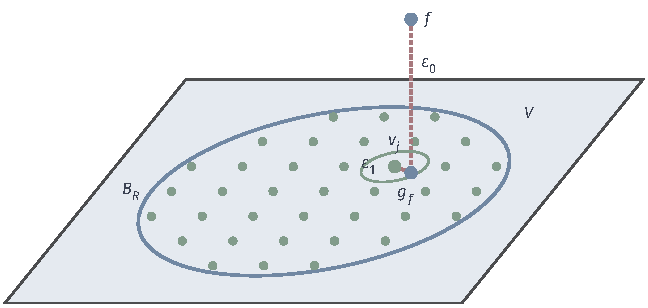
\includegraphics[width=109.7mm]{figures/04-spaces-measures-and-geometry/03-function-spaces/tikz/fcover-two-step/figure.pdf}
  \caption{两步覆盖的几何图景。平面是$n$维子空间$V$，蓝色椭圆是其中半径$R$的闭球，绿点是该球的$\varepsilon_1$网。$f$在$V$之外，先走到$V$中的近似$g_f$（红色虚线，长度不超过$\varepsilon_0$），再走到最近的网点$v_j$（红色实线，长度不超过$\varepsilon_1$）。}
  \label{fig:fcover-two-step}
\end{BookInlineFigure}

图~\ref{fig:fcover-two-step}画出了这两步。定理的两个前提分工明确。$\varepsilon_0$是统一逼近误差，它要求同一个$V$对整类有效，这是“存在$V$，对所有$f$”的量词次序；$R$限定近似所在的有界区域，使有限维覆盖可以进行。

对式~\eqref{eq:fcover-finite-dimensional}取对数，度量熵不超过$n\log(1+2R/\varepsilon_1)$。$n$取代了上一节的节点数，所以有限维表示的度量熵按$n\log(1/\varepsilon_1)$增长。复值函数空间可以看作实空间处理，$n$维复子空间的实维数是$2n$，指数相应换成$2n$。

\paragraph{范数界与系数界}

用范数表述时，界$R$几乎是自动的：若$\lVert f\rVert\leq B$，则$\lVert g_f\rVert\leq B+\varepsilon_0$。但实际存储的是某组基$\varphi_1,\ldots,\varphi_n$下的系数，量化的是系数而不是抽象的子空间元素，这时需要的是系数一致有界。

设$g_\theta=\sum_{i=1}^n\theta_i\varphi_i$，$\lvert\theta_i\rvert\leq\beta$，误差取一致范数，并记$\Lambda=\sup_x\sum_i\lvert\varphi_i(x)\rvert$。逐点估计，得到
\[
 \lVert g_\theta-g_{\theta'}\rVert_\infty\leq\Lambda\max_i\lvert\theta_i-\theta'_i\rvert .
\]
把每个系数量化到间距$2\varepsilon_1/\Lambda$的刻度上，按式~\eqref{eq:fcover-levels}的取法，每个系数有$\lceil\beta\Lambda/\varepsilon_1\rceil$种取值，得到至多$\lceil\beta\Lambda/\varepsilon_1\rceil^n$个代表，每个近似$g_f$与某个代表相差不超过$\varepsilon_1$。

系数界与范数界可以相差很大，差别来自基的选取。这和有限维的斜坐标系一样：两个基向量几乎平行时，同一个向量的坐标可能很大。在$C[0,1]$中取$\varphi_1=1$、$\varphi_2=1+\delta x$（$0<\delta<1$），则
\[
 x=\frac{\varphi_2-\varphi_1}\delta .
\]

函数$x$的一致范数是$1$，在这组基下的系数却是$(-1/\delta,1/\delta)$，$\delta$越小越大。取$\delta=0.01$、$\varepsilon_1=0.1$，用这组基存$x$需要$\beta=100$、$\Lambda=2.01$，每个系数的刻度数是
\[
 \Bigl\lceil\frac{100\cdot2.01}{0.1}\Bigr\rceil=2010 .
\]
而基$(1,x)$下系数只有$(0,1)$，$\beta=1$、$\Lambda=2$，每个系数$\lceil2/0.1\rceil=20$种取值就够。

两组基张成同一个子空间，覆盖数的范数版本不受影响。按系数量化时，几乎线性相关的基会让刻度数膨胀。所以用系数构造覆盖，必须核对系数本身的一致上界，不能只看函数的范数。

\paragraph{正弦级数类的例子}

现在给出一个系数列真正起作用的例子。取$C[0,1]$中的函数类
\begin{equation}
 \mathcal F=\Bigl\{f(x)=\sum_{k\geq1}a_k\sin(k\pi x):\ \sum_{k\geq1}k\lvert a_k\rvert\leq1\Bigr\}.
 \label{eq:fcover-sine-class}
\end{equation}
由于$\sum_k\lvert a_k\rvert\leq1$，级数一致收敛，每个成员都是连续函数。条件$\sum_kk\lvert a_k\rvert\leq1$让靠后的系数整体变小，这正是本节要的“尾部可舍”。

取$V_n$为$\sin(k\pi x)$（$1\leq k\leq n$）张成的子空间，$g_f$为前$n$项部分和。当$k>n$时$\lvert a_k\rvert\leq(k/n)\lvert a_k\rvert$，所以尾项满足
\[
 \lVert f-g_f\rVert_\infty\leq\sum_{k>n}\lvert a_k\rvert\leq\frac1n\sum_{k>n}k\lvert a_k\rvert\leq\frac1n .
\]
部分和本身的范数不超过系数绝对值之和，所以$\lVert g_f\rVert_\infty\leq1$。

用一个具体成员核对。$f(x)=\tfrac12\sin(\pi x)+\tfrac16\sin(3\pi x)$满足$1\cdot\tfrac12+3\cdot\tfrac16=1$，取$n=2$时被舍去的是$\tfrac16\sin(3\pi x)$，误差为$1/6$，不超过$1/n=1/2$。

所以定理~\ref{thm:fcover-finite-dimensional}的前提在$\varepsilon_0=1/n$、$R=1$下成立。给定$\varepsilon$，取$n=\lceil2/\varepsilon\rceil$与$\varepsilon_1=\varepsilon/2$，则$\varepsilon_0+\varepsilon_1\leq\varepsilon$，于是
\begin{equation}
 \log N_{C[0,1]}(\varepsilon,\mathcal F)\leq\Bigl\lceil\frac2\varepsilon\Bigr\rceil\log\Bigl(1+\frac4\varepsilon\Bigr).
 \label{eq:fcover-sine-entropy}
\end{equation}
例如$\varepsilon=1/2$时$n=4$，上界为$4\ln9\approx8.79$；$\varepsilon=0.1$时$n=20$，上界为$20\ln41\approx74.3$。

式~\eqref{eq:fcover-sine-entropy}与上一节一维Lipschitz类的式~\eqref{eq:fcover-entropy-bound}同为$\varepsilon^{-1}\log(1/\varepsilon)$的形式。这不是巧合：逐项求导得$\lvert f'\rvert\leq\pi$，$\mathcal F$本身含于一个Lipschitz类。两种构造从不同的结构出发，一个截取取值列，一个截取系数列，得到同样形式的计数。表~\ref{tab:fcover-two-lists}对比了两条路线。

\begin{BookInlineTable}
  \centering
  \begin{tabular}{@{}lll@{}}
    \toprule
    & 取值列 & 系数列\\
    \midrule
    下标 & 网格节点$v$ & 基函数编号$k$\\
    利用的约束 & 相邻节点相差至多$L/m$ & 舍去的尾部不超过$\varepsilon_0$\\
    有效坐标数 & $(m+1)^d$ & $n$\\
    每个坐标 & $T$个刻度 & 有限维球覆盖\\
    度量熵上界 & 式~\eqref{eq:fcover-entropy-bound} & $n\log(1+2R/\varepsilon_1)$\\
    \bottomrule
  \end{tabular}
  \caption{两条路线对比。两者都把函数看作一列数，都把无穷多个坐标压缩成有限个有效坐标，区别在于压缩所依据的约束。}
  \label{tab:fcover-two-lists}
\end{BookInlineTable}

\paragraph{从多个子空间中选择}

若不要求所有成员共用一个子空间，而允许每个成员从$J$个候选子空间$V_1,\ldots,V_J$中挑选一个（各为$n$维，前提中的$\varepsilon_0$与$R$相同），就对每个候选子空间分别构造覆盖，再取并集：
\begin{equation}
 \log N_E(\varepsilon_0+\varepsilon_1,\mathcal F)\leq\log J+n\log\Bigl(1+\frac{2R}{\varepsilon_1}\Bigr).
 \label{eq:fcover-many-subspaces}
\end{equation}

选择的自由要用$\log J$支付。例如从$D$个固定的基函数中任选$n$个，$J=\binom Dn\leq D^n$，度量熵多出至多$n\log D$。取$D=100$、$n=5$，有$J=75\,287\,520$，$\ln J\approx18.1$，而上界$n\ln D\approx23.0$。

候选子空间的个数必须受控。若候选子空间是一个连续参数族，例如所有平移$\varphi(x-t)$各自张成的一维子空间，$J$为无穷，上面的并集论证就失效，需要另行覆盖参数$t$。怎样构造满足这些前提的有限表示，固定子空间与自适应选择的误差怎样比较，是第~\ref{chap:function-approximation}章的问题。
